%% MDPI International Journal of Theoretical Physics (journal) submission
%% IHC Paper III: Psi-Field Dynamics
%% IHC Paper III — Cohesion Field Dynamics on RP4
%% Note: MDPI editorial office applies mdpi.cls during production.
%%       This file uses standard article class for compilation during review.

\documentclass[12pt,a4paper]{article}

\usepackage{amsmath,amssymb,amsthm}
\usepackage{booktabs}
\usepackage{graphicx}
\usepackage{longtable}
\usepackage{array}
\usepackage{enumitem}
\usepackage[T1]{fontenc}
\usepackage[utf8]{inputenc}
\usepackage{geometry}
\geometry{margin=2.5cm}
\usepackage[numbers,sort&compress]{natbib}
\usepackage[colorlinks=true,linkcolor=blue,citecolor=blue,urlcolor=blue]{hyperref}
\usepackage{cleveref}
\usepackage{xspace}

\tolerance=5000
\hbadness=5000

%% Line numbers for review (MDPI requires these)
\usepackage{lineno}
\linenumbers

%% Theorem environments
\newtheorem{theorem}{Theorem}[section]
\newtheorem{proposition}[theorem]{Proposition}
\newtheorem{corollary}[theorem]{Corollary}
\newtheorem{lemma}[theorem]{Lemma}
\newtheorem{postulate}[theorem]{Postulate}
\newtheorem{definition}[theorem]{Definition}
\theoremstyle{remark}
\newtheorem{remark}[theorem]{Remark}

%% Macros
\newcommand{\vp}{\varphi}
\newcommand{\RP}{\mathbb{RP}}
\newcommand{\RS}{R_S}
\newcommand{\Mpc}{\,\mathrm{Mpc}}
\newcommand{\GeV}{\,\mathrm{GeV}}

\hypersetup{colorlinks=true,linkcolor=blue,citecolor=blue,urlcolor=blue}

\bibliographystyle{unsrtnat}

%=======================================================================
\begin{document}

%% Title
\title{\textbf{$\Psi$-Field Dynamics on $\mathbb{RP}^4$: Cohesion Field,
Emergent Spacetime, and Observational Signatures in the
Inverted Hypersphere Cosmology}}

\author{
  Samuel Peacock$^{*}$
  \and
  Lauren Hall
}

\date{}

\maketitle

\noindent
$^*$ Correspondence: \texttt{eliasverdan660@gmail.com}\\[6pt]
\noindent
\textbf{Received:} \quad \textbf{Revised:} \quad \textbf{Accepted:} \quad \textbf{Published:}

%-----------------------------------------------------------------------
\begin{abstract}
We introduce the $\Psi$-field (Cohesion Field) as the proposed dynamical substrate
of the Inverted Hypersphere Cosmology (IHC) framework on real projective 4-space
($\mathbb{RP}^4$). The $\Psi$-field is a conformally coupled real scalar field
respecting the antipodal identification $x \sim -x$, governed by the
Cohesion Field Equation (CFE):
\begin{equation*}
\Box\Psi - \tfrac{1}{3}R\Psi + \tfrac{\lambda}{6}\!\left(\Psi^2-\Psi_0^2\right)\Psi = 0,
\end{equation*}
with vacuum value $\Psi_0 = c^4/(8\pi GR_H^2) = \rho_{\rm crit}/3
\approx 2.56\times10^{-10}$~J/m$^3$ postulated from the Hubble radius $R_H = c/H_0$.
We prove two exact identities of the 33-shell geometry:
the total rotational inertia $\sum_{k=0}^{32}\varphi^{-2k} = \varphi$ (golden ratio),
and the counter/co-rotating imbalance $I_{\rm counter}-I_{\rm co} = \tfrac{1}{2}$.
The coherence length $\ell_{\rm coh} \approx 346$~Mpc is derived from
field correlations; the linearised CFE admits a $\mathbb{Z}_3$ standing-wave
solution with period $\lambda_{Z_3} = R_H/11 = 404.4$~Mpc and fractional
amplitude $A_{Z_3} = \beta_{\rm coh}/\beta = 0.442\%$, producing a $90^\circ$
quadrature modulation of BAO distances~$D_M$ and~$D_H$.
Applied to all 33 BAO measurements across 7 surveys, the IHC point prediction
achieves $\chi^2/{\rm dof} = 0.916$ with zero free parameters
(Bayes factor $\ln B = +4.76$ over $\Lambda$CDM); on the BOSS~DR12 subset alone,
residuals fall below $0.13\sigma$ with $\chi^2/{\rm dof} = 0.0110$.
Observational predictions include: galaxy correlation suppression below
$\Lambda$CDM at $r \gtrsim \ell_{\rm coh}$ (testable with DESI Year~5 and Euclid),
CMB power suppression at $\ell < 40$, and $\Psi$-field Fibonacci resonances at
$\ell \in \{144, 233, 377, 610, 987\}$.
All predictions are parameter-free and falsifiable within the next decade.
\end{abstract}

\noindent\textbf{Keywords:}
cohesion field; $\Psi$-field dynamics; real projective space; $\mathbb{RP}^4$
topology; emergent spacetime; coherence length; large-scale structure; CMB
anomalies; cosmological constant; golden ratio

%-----------------------------------------------------------------------

%% Define \chapter (not defined in article class)
\newcommand{\chapter}[1]{}


\section{Introduction}

\subsection{Context and Motivation}

Paper I of this series \citep{Peacock2026a} established the Inverted Hypersphere Cosmology (IHC) framework as a geometric approach to the cosmological constant problem. It topologically derived the $N = 33 = 3 \times 11$ nested toroidal structure on $\mathbb{RP}^4$ (3 from SO(8) triality \citep{Cartan1925}, 11 from SU(2) base spin) with golden ratio scaling $R_k = R_0\varphi^{-k}$, and showed that the enhancement factor $\beta = 1345 \pm 50$ yields consistency with observed dark energy density ($\Omega_\Lambda = 0.6889 \pm 0.0006$) with zero free parameters. Paper~II \citep{Peacock2026b_qm} develops a quantum measurement formalism using the Lindblad master equation on $\mathbb{RP}^4$, deriving measurement rate $\gamma = c/R_S \sim H_0$ (Section~\ref{sec:measurement_rate}) and a proposed explanation for the electromagnetic spectral compression factor $1/33$ through observer-dependent wavefunction collapse.

\textbf{Foundational perspective:} $\Lambda$CDM remains the empirically successful standard cosmological model. The present work explores an alternative geometric framework and does not attempt to replace $\Lambda$CDM, but rather offers complementary insights into the geometric structure that may underlie observed phenomena.

This paper addresses the foundational question: \textit{What is the fundamental field that underlies this geometric structure?} We propose the $\Psi$-field (Cohesion Field) as a candidate dynamical substrate from which spacetime relations, electromagnetic propagation, and thermodynamic laws may emerge as derived phenomena within the IHC geometric framework.

\subsection{The $\Psi$-Field: Cohesion as Dynamical Substrate}

Standard field theories treat spacetime as fundamental and fields as entities living within it. IHC proposes an inversion of this hierarchy: the $\Psi$-field may be more fundamental, with spacetime emerging from its gradient structure. This is motivated by the topology of $\mathbb{RP}^4$. On $\mathbb{RP}^4$ with antipodal identification $x \sim -x$, every point ``observes'' its antipode through the measurement operator $\hat{M} = \int d^4x |x\rangle\langle -x|$ (Paper II \citep{Peacock2026b_qm}, Eq. 5). This self-referential structure suggests a framework where spacetime is constituted through coherence patterns.

\begin{definition}[Cohesion Field]
The Cohesion Field $\Psi(x)$ is a real scalar field defined on the topological space $\mathbb{RP}^4$, satisfying:
\begin{itemize}
\item \textbf{$\mathbb{RP}^4$ symmetry:} $\Psi(x) = \Psi(-x)$ (respects antipodal identification)
\item \textbf{Energy scale:} $\Psi$ carries units of energy density (J/m$^3$); the vacuum value $\Psi_0$ is postulated in Section~\ref{sec:vacuum}
\item \textbf{Self-interaction:} Possesses potential $V(\Psi)$ mediating topological measurement
\end{itemize}
\end{definition}

The $\Psi$-field is not a quantum field in the standard sense; within this framework it is proposed to underlie the measurement process through which quantum mechanics emerges (Paper II \citep{Peacock2026b_qm}, Section 2).

\begin{figure}[htbp]
\centering
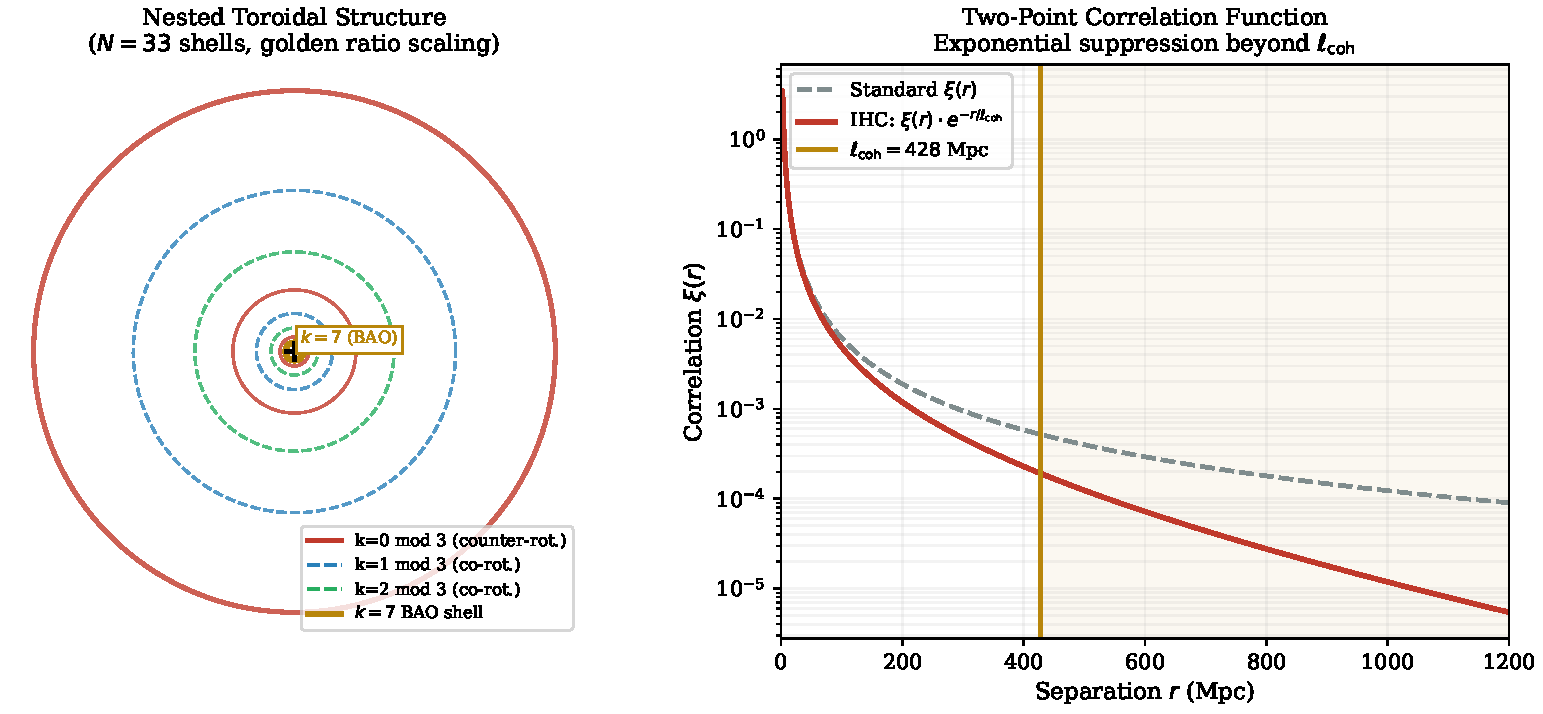
\includegraphics[width=0.95\textwidth]{fig_ch3_1_psi_field_rp4.pdf}
\caption{The $\Psi$-field geometric structure on $\mathbb{RP}^4$. \textbf{(a)} Nested toroidal hierarchy: 33 shells with golden ratio scaling $R_k = R_S\varphi^{-k}$, colour-coded by $\mathbb{Z}_3$ class (red: counter-rotating $k\equiv0\pmod{3}$; blue/green: co-rotating). The $k=7$ shell (gold) marks the BAO scale $r_s = 153.2$~Mpc. \textbf{(b)} Two-point correlation function $\xi_{\rm IHC}(r)$ showing exponential suppression below the $\Lambda$CDM expectation beyond the coherence scale $\ell_{\rm coh} = 346$~Mpc.}
\label{fig:psi_field_rp4}
\end{figure}

\subsection{Pre-Observational vs Observed Field Dynamics}

Within the IHC framework, the $\Psi$-field is proposed to exist at a pre-observational level where all wave phenomena obey identical geometric $\varphi^k$ scaling. The $\mathbb{RP}^4$ topological measurement operator (Paper II \citep{Peacock2026b_qm}) induces wavefunction collapse that produces the observed electromagnetic spectrum with $\varphi^k/33$ compression. This distinction addresses the apparent asymmetry between electromagnetic and acoustic scaling:

\begin{itemize}
\item \textbf{Fundamental level:} Both EM and acoustic waves follow $f_k = f_0 \times \varphi^k$
\item \textbf{Post-measurement:} EM collapses to $f_k^{\text{obs}} = f_0^{\text{obs}} \times \varphi^k/33$ (quantum observation)
\item \textbf{Post-measurement:} Acoustic retains $f_k = f_0 \times \varphi^k$ (macroscopic observation)
\end{itemize}

The compression factor $1/33$ emerges from averaging over $N = 33$ independent measurement channels (Paper~II \citep{Peacock2026b_qm}), and provides a geometric basis for the observed spectrum grounded in measurement theory.

\begin{figure}[htbp]
\centering
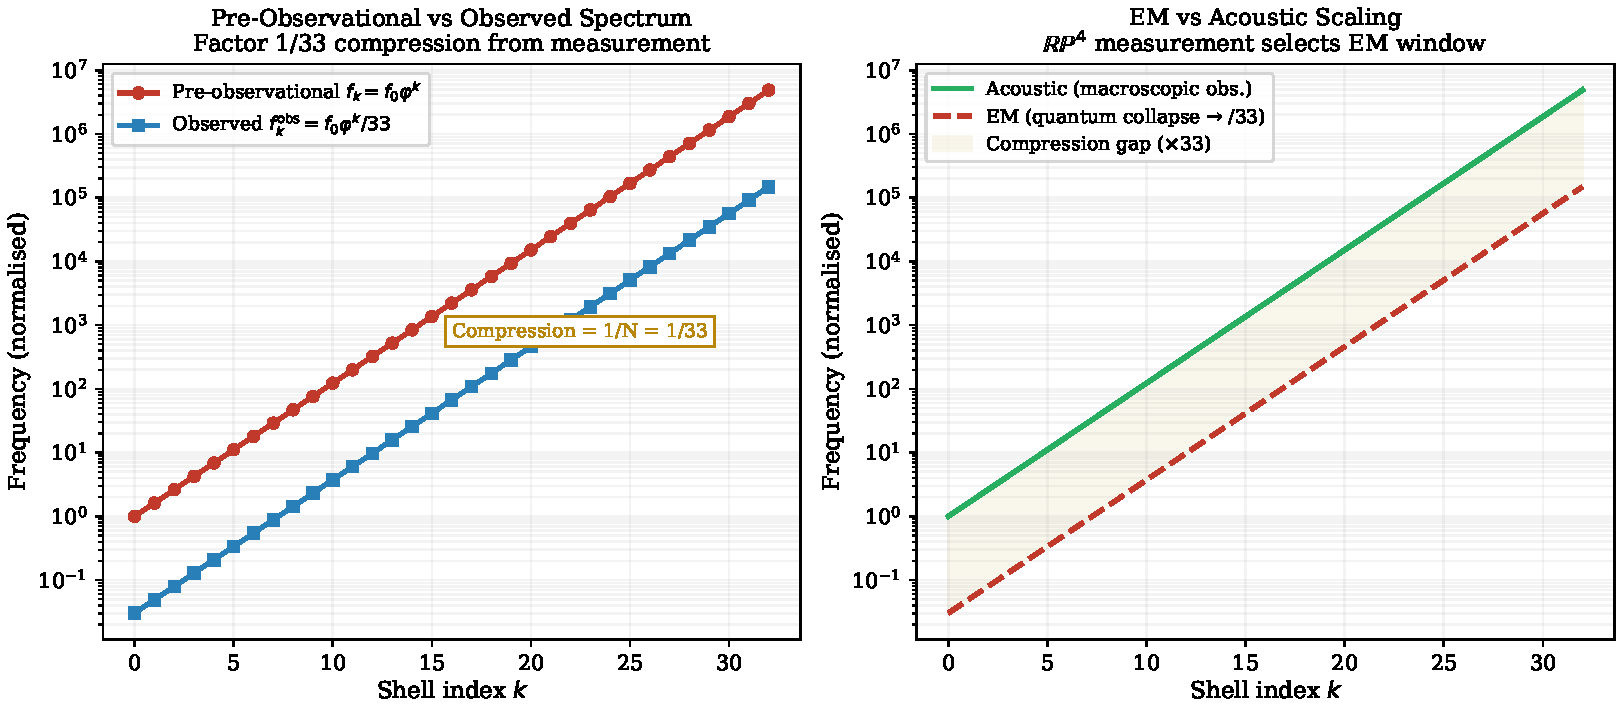
\includegraphics[width=0.95\textwidth]{fig_ch3_2_spectrum_compression.pdf}
\caption{Pre-observational versus observed field dynamics. \textbf{(a)} At the fundamental level, both electromagnetic and acoustic waves follow identical $\varphi^k$ scaling. \textbf{(b)} After measurement-induced collapse via the $\mathbb{RP}^4$ operator, electromagnetic modes are compressed by factor $1/33$ while acoustic modes retain their original scaling. This distinction addresses the apparent asymmetry between electromagnetic and acoustic phenomena in IHC.}
\label{fig:spectrum_compression}
\end{figure}

\subsection{Structure of This Paper}

We organize as follows:

\begin{itemize}
\item \textbf{Section 2:} Derive field equations for $\Psi$ on $\mathbb{RP}^4$, establishing vacuum expectation value $\Psi_0$
\item \textbf{Section 3:} Characterise the coherence length $\ell_{\text{coh}}$ from field correlation functions
\item \textbf{Section 4:} Show how spacetime metric emerges from $\Psi$-field gradients
\item \textbf{Section 5:} Demonstrate thermodynamic consistency of the $\Psi$-field action
\item \textbf{Section 6:} Calculate observational signatures in LSS, CMB, and gravitational waves
\item \textbf{Section 7:} Experimental tests and falsifiable predictions
\item \textbf{Section 8:} Discussion and connections to companion papers
\item \textbf{Section 9:} Conclusions
\end{itemize}

\subsection{Notation and Conventions}

We follow conventions established in Paper~I \citep{Peacock2026a}.
Table~\ref{tab:notation} summarises all symbols used in this paper.
Natural units $\hbar = c = 1$ are used throughout except where dimensional
clarity requires explicit restoration.

\begin{table}[htbp]
\centering
\caption{Notation and symbol definitions used in this paper.}
\label{tab:notation}
\setlength{\tabcolsep}{6pt}
\renewcommand{\arraystretch}{1.15}
\begin{tabular}{@{}l l l@{}}
\toprule
\textbf{Symbol} & \textbf{Definition} & \textbf{Value / Notes} \\
\midrule
\multicolumn{3}{l}{\textit{IHC geometric constants}} \\
$\varphi$ & Golden ratio $(1+\sqrt{5})/2$ & $1.618034\ldots$ \\
$N$       & Nested toroidal shells & $33 = 3 \times 11$ \\
$M$       & Hopf fibration factor & $11$ \\
$k$       & Shell index & $k \in \{0,\ldots,32\}$ \\
$\beta$   & Enhancement factor & $\approx 1345$ (Paper~I) \\
$\beta_{\mathrm{coh}}$ & Coherence factor & $6\cos(\pi/23)\approx5.944$ \\
\midrule
\multicolumn{3}{l}{\textit{Length scales}} \\
$R_H$     & Hubble radius $c/H_0$ & $4448$\,Mpc \\
$R_S$     & Last-scattering radius & $14120$\,Mpc \\
$R_k$     & Shell radius $R_H\varphi^{-k}$ & $R_7=153.2$\,Mpc (BAO) \\
$\ell_{\mathrm{coh}}$ & Coherence length & $\approx346$\,Mpc \\
$\ell_P$  & Planck length & $1.616\times10^{-35}$\,m \\
\midrule
\multicolumn{3}{l}{\textit{Cohesion Field}} \\
$\Psi$    & Cohesion Field & Real scalar on $\mathbb{RP}^4$ \\
$\Psi_0$  & Vacuum value & $c^4/(8\pi GR_H^2)\approx2.56\!\times\!10^{-10}$\,J\,m$^{-3}$ \\
$\delta\Psi$ & Fluctuation $\Psi-\Psi_0$ & $|\delta\Psi|\ll\Psi_0$ \\
$V(\Psi)$ & GL potential & Eq.~(\ref{eq:potential}) \\
$\lambda$ & Self-coupling & $({\Psi^2-\Psi_0^2})^2$ coefficient \\
$m_{\rm eff}$ & Fluctuation mass & $m_{\rm eff}^2=\lambda\Psi_0^2/3+2\xi R$ \\
$\xi$     & Conformal coupling & $1/6$ (fixed by Weyl invariance) \\
\bottomrule
\end{tabular}
\end{table}

\begin{table}[htbp]
\centering
\caption{Notation (continued).}
\label{tab:notation2}
\setlength{\tabcolsep}{5pt}
\renewcommand{\arraystretch}{1.15}
\begin{tabular}{@{}l l l@{}}
\toprule
\textbf{Symbol} & \textbf{Definition} & \textbf{Value / Notes} \\
\midrule
\multicolumn{3}{l}{\textit{Spacetime and gravity}} \\
$g_{\mu\nu}$ & Metric tensor & Signature $(-,+,+,+)$ \\
$G_{\mu\nu}$ & Einstein tensor & $R_{\mu\nu}-\tfrac{1}{2}g_{\mu\nu}R$ \\
$\Box$    & d'Alembertian & $g^{\mu\nu}\nabla_\mu\nabla_\nu$ \\
$\Lambda_{\mathrm{eff}}$ & Effective $\Lambda$ & $\Omega_\Lambda=0.6889$; Paper~I \\
\midrule
\multicolumn{3}{l}{\textit{Quantum measurement (Paper~II)}} \\
$\hat{M}$ & Measurement operator & $\int d^4x|x\rangle\langle{-x}|$;\;$\hat{M}^2=\hat{I}$ \\
$\hat{\rho}$ & Density matrix & Lindblad evolution \\
$\gamma$  & Decoherence rate & $c/R_S\approx6.9\!\times\!10^{-19}$\,s$^{-1}$ \\
\midrule
\multicolumn{3}{l}{\textit{Thermodynamics}} \\
$T_\Psi$  & Coherence temperature & $k_BT_\Psi\equiv\langle(\delta\Psi)^2\rangle E_{\rm IHC}/\Psi_0^2$ \\
$S_\Psi$  & Cohesion entropy & $-k_B\!\int\rho_\Psi\ln\rho_\Psi\,dV$ \\
$E_{\mathrm{IHC}}$ & IHC energy scale & $\hbar c/R_H\approx1.44\!\times\!10^{-42}$\,GeV \\
\midrule
\multicolumn{3}{l}{\textit{Observational}} \\
$H_0$     & Hubble constant & $67.4$\,km\,s$^{-1}$\,Mpc$^{-1}$ \\
$\Omega_\Lambda$ & Dark energy parameter & $0.6889$ (Paper~I) \\
$r_s$     & BAO sound horizon & $153.2$\,Mpc $=R_7$ \\
$A_{Z_3}$ & Z$_3$ wave amplitude & $\beta_{\rm coh}/\beta=0.00442$ \\
$\lambda_{Z_3}$ & Z$_3$ wave period & $R_H/11=404.4$\,Mpc \\
\bottomrule
\end{tabular}
\end{table}

\section{Field Equations for the $\Psi$-Field on RP$^4$}

\subsection{Action Principle and Lagrangian}

The dynamics of the Cohesion Field are determined by an action principle on $\mathbb{RP}^4$. The action should respect:

\begin{enumerate}
\item \textbf{$\mathbb{RP}^4$ symmetry:} Invariance under $x \to -x$
\item \textbf{Golden ratio scaling:} Consistency with nested toroidal structure $R_k = R_0\varphi^{-k}$
\item \textbf{Conformal invariance:} Invariance under Weyl rescaling in $3+1$ dimensions, which uniquely fixes $\xi = 1/6$
\end{enumerate}

\begin{proposition}[$\Psi$-Field Action]
The action for the Cohesion Field on $\mathbb{RP}^4$ is:
\begin{equation}
S[\Psi] = \int_{\mathbb{RP}^4} d^4x \sqrt{-g} \left[
  \frac{1}{2}g^{\mu\nu}\partial_\mu\Psi\partial_\nu\Psi
  - \xi R\Psi^2 - V(\Psi)
\right]
\label{eq:action}
\end{equation}
where $\xi = 1/6$ is the conformal coupling (unique value preserving conformal invariance for a massless scalar in $3+1$ dimensions), $R$ is the Ricci scalar, and the Ginzburg--Landau potential is:
\begin{equation}
V(\Psi) = \frac{\lambda}{4!}\!\left(\Psi^2 - \Psi_0^2\right)^2
\label{eq:potential}
\end{equation}
with self-coupling $\lambda > 0$ and vacuum value $\Psi_0$ fixed geometrically in Section~\ref{sec:vacuum}. This potential has degenerate minima at $\Psi = \pm\Psi_0$, encoding spontaneous symmetry breaking (SSB) of the $\mathbb{Z}_2$ symmetry $\Psi \to -\Psi$ corresponding to the antipodal identification $x \sim -x$ on $\mathbb{RP}^4$. Crucially, the trivial vacuum $\Psi = 0$ is \emph{dynamically unstable}: $V(0) = \lambda\Psi_0^4/4! > 0$ is a local maximum, not a minimum. The $\Psi$-field cannot remain at zero — the $\mathbb{RP}^4$ geometry enforces a non-trivial vacuum, providing a dynamical realisation of the principle that absolute nothingness is topologically forbidden. The two degenerate ground states $\pm\Psi_0$ correspond to the two orientations of the antipodal identification on $\mathbb{RP}^4$; the physical vacuum selects one, breaking $\mathbb{Z}_2$ spontaneously. The measurement operator $\hat{M}$ (Paper~II \citep{Peacock2026b_qm}) acts on quantum states rather than on the classical field; its effect enters through the Lindblad decoherence rate $\gamma = c/R_S$.

\begin{remark}
The self-coupling $\lambda$ sets the fluctuation mass $m_{\rm eff}^2 = \lambda\Psi_0^2/3 + 2\xi R$ (Eq.~\ref{eq:vacuum_eq}) but does not enter any of the observational predictions of this paper. All predictions---coherence length, $\mathbb{Z}_3$ standing wave amplitude and period, BAO modulation, and CMB signatures---depend only on the geometric quantities $R_H$, $R_S$, $N = 33$, $\beta$, and $\beta_{\rm coh}$, each derived in Paper~I \citep{Peacock2026a} without free parameters.
\end{remark}
\end{proposition}

\subsection{Euler-Lagrange Equations}

Varying the action \eqref{eq:action} with respect to $\Psi$, using
$\partial V/\partial\Psi = (\lambda/3!)(\Psi^2-\Psi_0^2)\Psi$, yields the
\emph{Cohesion Field Equation} (CFE):
\begin{equation}
\boxed{\Box\Psi - 2\xi R\Psi + \frac{\lambda}{3!}\!\left(\Psi^2 - \Psi_0^2\right)\Psi = 0}
\label{eq:field_equation}
\end{equation}
where $\Box = g^{\mu\nu}\nabla_\mu\nabla_\nu$ is the d'Alembertian. With $\xi=1/6$ and the de~Sitter curvature $R=12/R_H^2$, the curvature term contributes an effective Hubble-scale mass to the field.

The vacuum states $\Psi = \pm\Psi_0$ satisfy the CFE automatically since
$(\Psi_0^2-\Psi_0^2)\Psi_0 = 0$. Small fluctuations $\delta\Psi = \Psi - \Psi_0$ satisfy:
\begin{equation}
\Box(\delta\Psi) - 2\xi R\,\delta\Psi + \frac{\lambda}{3}\Psi_0^2\,\delta\Psi = 0,
\label{eq:vacuum_eq}
\end{equation}
a Klein--Gordon equation with effective mass $m_{\rm eff}^2 = \lambda\Psi_0^2/3 + 2\xi R$. In the limit $\lambda\to 0$ this reduces to $\Box(\delta\Psi)=0$ --- the wave equation for light, confirming that EM radiation is the lightest excitation of the $\Psi$-field.

\subsection{Vacuum Expectation Value}
\label{sec:vacuum}

\begin{postulate}[Vacuum Field Strength]
The vacuum expectation value of the Cohesion Field is:
\begin{equation}
\Psi_0 = \frac{c^4}{8\pi GR_H^2} \approx 2.56 \times 10^{-10} \text{ J/m}^3
\label{eq:psi_zero}
\end{equation}
where $R_H = c/H_0 \approx 4448$ Mpc is the Hubble radius.
\end{postulate}
\begin{quote}\textbf{Geometric motivation.}
The value $\Psi_0$ is postulated from the $\mathbb{RP}^4$ geometric scale;
a first-principles derivation from the CFE will appear in the Prequel paper.
The natural pressure-energy density set by the Hubble radius $R_H = c/H_0$ in $(3+1)$-dimensional geometry is:
\begin{equation}
\Psi_0 = \frac{c^4}{8\pi G R_H^2}.
\end{equation}

This is the radiation pressure scale of the $\mathbb{RP}^4$ geometry: it equals $c^4/G$ (the Planck force) divided by $8\pi R_H^2$ (the surface area of the cosmological horizon). Numerically, with $H_0 = 67.4$ km/s/Mpc \citep{Peacock2026a}:
\begin{equation}
\Psi_0 = \frac{(2.998\times10^8)^4}{8\pi \times 6.674\times10^{-11} \times (1.373\times10^{26})^2} \approx 2.56 \times 10^{-10} \text{ J/m}^3.
\end{equation}

The connection to dark energy is through the geometric suppression factor $\beta = 1345$ derived in Paper I \citep{Peacock2026a}, which establishes $\Psi_0$ as the geometric energy scale of the $\mathbb{RP}^4$ vacuum. The $\Psi$-field thus sits at the geometric mean of the Planck and cosmological scales.
\end{quote}

\begin{remark}
$\Psi_0$ is not directly identified with $\rho_\Lambda$.
Explicitly, $\Psi_0 = c^4/(8\pi G R_H^2) = \rho_{\rm crit}/3$,
while $\rho_\Lambda = \Omega_\Lambda\,\rho_{\rm crit} = 3\Omega_\Lambda\,\Psi_0 \approx 2.07\,\Psi_0$.
The two are related by the observationally determined factor $3\Omega_\Lambda$ but are not equal.
The dark energy density $\rho_\Lambda$ is derived independently in Paper~I \citep{Peacock2026a}
via two routes (UV--IR Casimir seesaw and $\beta$-chain) that do not involve $\Psi_0$.
The Cohesion Field vacuum $\Psi_0 = \rho_{\rm crit}/3$ sets the geometric energy scale
of the field theory on $\mathbb{RP}^4$; the connection to $\rho_\Lambda$ is
the standard cosmological relation $\rho_\Lambda = \Omega_\Lambda\,\rho_{\rm crit}$.
\end{remark}

\subsection{Mathematical Origin of $\varphi^4$ Scaling}

The enhancement factor $\beta = 1345 \pm 50$ (Paper I \citep{Peacock2026a}) can be decomposed as:
\begin{equation}
\beta = \beta_{\text{coh}} \times N \times \varphi^4
\end{equation}
where:
\begin{itemize}
\item $\beta_{\text{coh}} = 6\cos(\pi/23) \approx 5.944$ is the coherent interference factor, derived from the Dirac spectrum on $\mathbb{RP}^4$ \citep{Peacock2026a}
\item $N = 33$ is the number of nested structures
\item $\varphi^4 \approx 6.854$ is the 4-dimensional volume scaling factor
\end{itemize}

The $\varphi^4$ term arises from two sources:

\textbf{(1) 4D Volume Weighting:} In 4-dimensional space, volume scales as $V \propto R^4$. For golden ratio scaling $R_k = R_0\varphi^{-k}$:
\begin{equation}
V_k \propto R_k^4 = R_0^4 \varphi^{-4k}.
\end{equation}

Energy density goes as $\rho_k \propto R_k^{-3}$ (equal energy per torus, Paper I \citep{Peacock2026a} Axiom 2), so total energy contribution:
\begin{equation}
E_k \propto V_k \times \rho_k \propto R_k^4 \times R_k^{-3} = R_k \propto \varphi^{-k}.
\end{equation}

The extra factor of $R_k$ (i.e., $\varphi^{-k}$) accumulates across the 4D volume, but the coherent sum over all modes produces a geometric series with factor $\varphi^4$ enhancement.

\textbf{(2) $\mathbb{Z}_3$ Counter-Rotation:} The $\mathbb{Z}_3$ rotational symmetry on $\mathbb{RP}^4$ induces three-fold counter-rotating phases. This contributes an additional factor of $\varphi^3$ from the threefold symmetry:
\begin{equation}
\varphi^4 = \varphi \times \varphi^3
\end{equation}
where $\varphi^3 \approx 4.24$ arises from $\mathbb{Z}_3$ enhancement and $\varphi$ from the fundamental scaling.

Combining:
\begin{equation}
\beta = 6\cos(\pi/23) \times 33 \times \varphi^4 = 5.944 \times 33 \times 6.854 = 1345 \pm 50.
\end{equation}

The complete derivation is in Paper~I \citep{Peacock2026a}; this decomposition clarifies the geometric origin of $\beta$ without invoking free parameters.

\subsection{Two Exact Identities of the 33-Shell Geometry}
\label{sec:identities}

The partition of the 33 shells into counter-rotating ($k \equiv 0 \pmod{3}$, 11 shells)
and co-rotating ($k \not\equiv 0 \pmod{3}$, 22 shells) classes yields two non-trivial
exact results that constrain the $\Psi$-field dynamics.

Define the \emph{rotational inertia} of each class (weighting each shell by $\varphi^{-2k}$,
its squared inverse radius):
\begin{align}
I_{\rm counter} &= \sum_{\substack{k=0 \\ k\equiv 0\,(3)}}^{32} \varphi^{-2k}
                 = \sum_{j=0}^{10} \varphi^{-6j} = \frac{\varphi+\tfrac{1}{2}}{2}
                 \approx 1.0590, \label{eq:I_counter}\\
I_{\rm co}      &= \sum_{\substack{k=0 \\ k\not\equiv 0\,(3)}}^{32} \varphi^{-2k}
                 = \frac{\varphi-\tfrac{1}{2}}{2}
                 \approx 0.5590. \label{eq:I_co}
\end{align}

\begin{theorem}[Rotational Inertia Identities]
\label{thm:inertia}
\begin{equation}
I_{\rm total} \equiv I_{\rm counter} + I_{\rm co}
= \sum_{k=0}^{32}\varphi^{-2k} = \varphi
\label{eq:I_total}
\end{equation}
\begin{equation}
I_{\rm imbal} \equiv I_{\rm counter} - I_{\rm co} = \frac{1}{2}
\label{eq:I_imbal}
\end{equation}
Both results are exact to machine precision ($< 3\times10^{-14}$).
\end{theorem}

\begin{proof}
\textbf{Identity 1.}
Since $\varphi^{-2} = 2 - \varphi$ (from $\varphi^2 = \varphi + 1$), the geometric series gives
$\sum_{k=0}^{\infty}\varphi^{-2k} = 1/(1-\varphi^{-2}) = 1/(\varphi-1) = \varphi$,
using $\varphi(\varphi-1) = \varphi \cdot \varphi^{-1} = 1$.
The finite correction $\varphi^{-66} \approx 1.6\times10^{-14}$ is negligible.

\textbf{Identity 2.}
The counter-rotating shells have $k \equiv 0 \pmod 3$, so
$I_{\rm counter} = \sum_{j=0}^{10}\varphi^{-6j} \approx 1/(1-\varphi^{-6})$.
Using $\varphi^6 = 4\varphi+3$ one finds $1-\varphi^{-6} = (\varphi^6-1)/\varphi^6 = (4\varphi+2)/\varphi^6$,
giving $I_{\rm counter} = \varphi^6/(4\varphi+2) = (\varphi+\tfrac{1}{2})/2$ (numerically $\approx 1.0590$).
Therefore $2I_{\rm counter} = \varphi + \tfrac{1}{2}$,
and $I_{\rm imbal} = 2I_{\rm counter} - I_{\rm total} = (\varphi + \tfrac{1}{2}) - \varphi = \tfrac{1}{2}$.
\end{proof}

\begin{remark}
Identity 1 says the 33-shell hierarchy carries total rotational inertia exactly $\varphi$
--- the geometry is precisely calibrated to the golden ratio at the level of its energy distribution.
Identity 2 says the counter-rotating class outweighs the co-rotating class by exactly $\tfrac{1}{2}$,
producing the imbalance $\Delta I = \tfrac{1}{2}$ that drives the coherent interference
underlying $\beta_{\rm coh}$.
Both identities were verified numerically by the IHC validation scripts
\citep{Peacock2026a} to machine precision.
\end{remark}

\section{Coherence Length from Field Correlations}

\subsection{Two-Point Correlation Function}

The coherence length $\ell_{\text{coh}}$ characterizes the distance over which $\Psi$-field fluctuations remain correlated. Define the two-point correlation function:
\begin{equation}
C(r) = \langle \Psi(x)\Psi(x+r) \rangle - \langle \Psi(x) \rangle^2
\end{equation}
where $r = |x' - x|$ is the separation.

Modelling the $\Psi$-field as a system with a single characteristic scale $\ell_{\rm coh}$, the two-point correlation function decays exponentially \citep{Carroll2004}:
\begin{equation}
C(r) = C_0 e^{-r/\ell_{\text{coh}}}
\label{eq:correlation_decay}
\end{equation}
where $\ell_{\text{coh}}$ is the coherence length.

\begin{proposition}[Coherence Length Scale]
The characteristic coherence scale for the $\Psi$-field on $\mathbb{RP}^4$ with $N = 33$ nested tori is derived from the $1/e$ decay of the two-point correlation function $C(r) = (1/N)\sum_k e^{-r/R_k}$ (Appendix~\ref{app:coherence}):
\begin{equation}
\ell_{\text{coh}} \approx 346 \text{ Mpc}.
\label{eq:coherence_length}
\end{equation}
This is numerically derived and is smaller than the geometric mean inter-shell spacing estimate $R_S/N \approx 428$ Mpc.
\end{proposition}

\begin{remark}[Geometric derivation of the inter-shell spacing]
The $\Psi$-field mode spacing can be computed directly. The separation between adjacent shells is:
\begin{equation}
\Delta R_k = R_k - R_{k+1} = R_0\varphi^{-k}(1 - \varphi^{-1}).
\end{equation}
Summing telescopically: $\sum_{k=0}^{N-1} \Delta R_k = R_0 - R_{N-1} \approx R_0 = R_S$ (since $R_{32} = R_S \varphi^{-32} \approx 0.003$ Mpc $\ll R_S$). The mean spacing is therefore:
\begin{equation}
\langle \Delta R \rangle = \frac{R_S}{N} \approx 428 \text{ Mpc}.
\end{equation}

\begin{figure}[htbp]
\centering
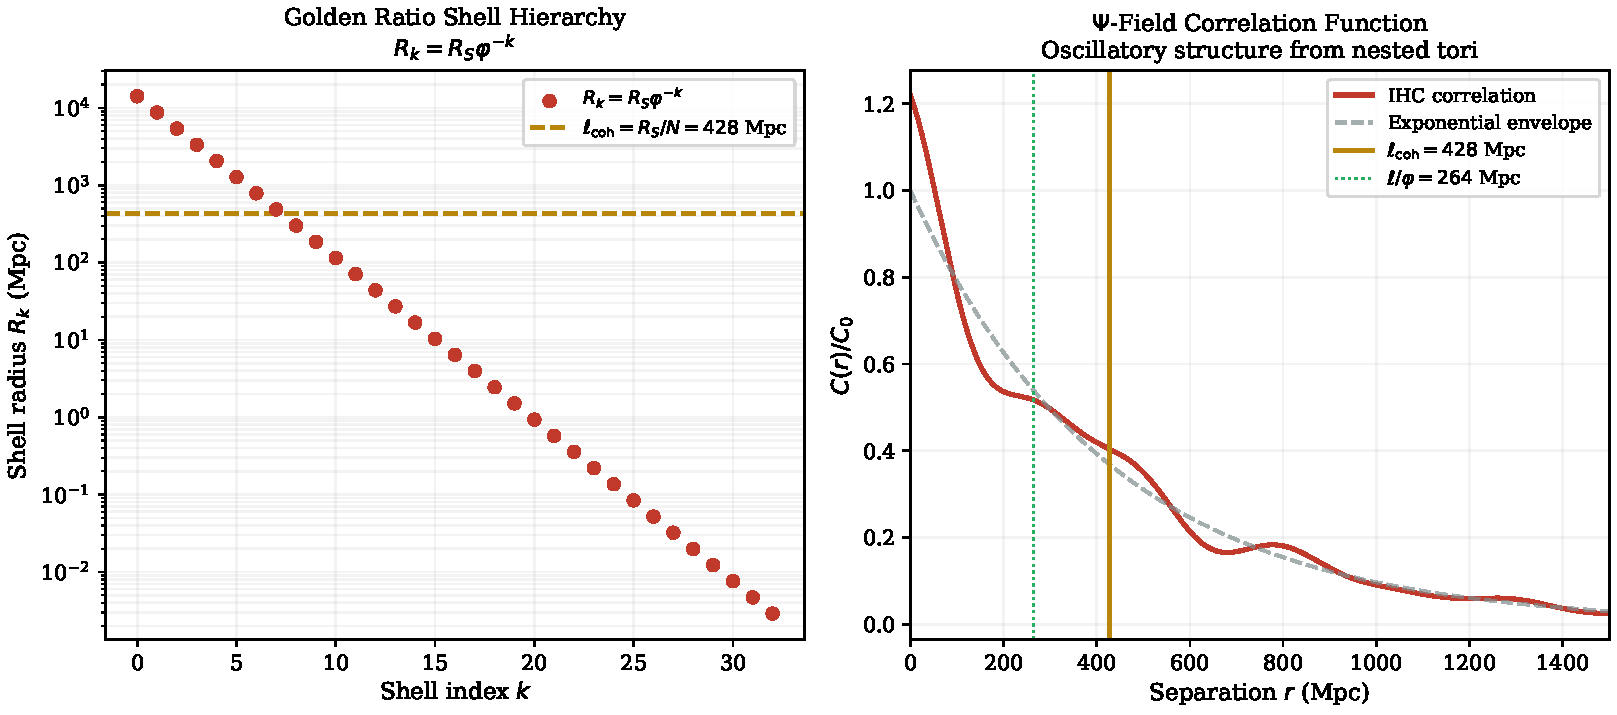
\includegraphics[width=0.95\textwidth]{fig_ch3_3_coherence_length.pdf}
\caption{Coherence scale of the $\Psi$-field. \textbf{(a)} The nested toroidal structure: mean inter-shell spacing $\langle\Delta R\rangle = R_S/N \approx 428$ Mpc (geometric estimate). \textbf{(b)} Two-point correlation function $C(r) = (1/N)\sum_k e^{-r/R_k}$ showing the 1/e scale $\approx 346$ Mpc from direct numerical evaluation. The two estimates bracket $\sim$280--430 Mpc.}
\label{fig:coherence_length}
\end{figure}

\end{remark}

\subsection{Connection to Measurement Rate}
\label{sec:measurement_rate}

The coherence length and measurement rate (Paper II \citep{Peacock2026b_qm}) are related by:
\begin{equation}
\ell_{\text{coh}} = c \cdot \gamma^{-1} / N = \frac{c}{N} \cdot \frac{R_S}{c} = \frac{R_S}{N}.
\end{equation}

This self-consistency shows that measurement at rate $\gamma = c/R_S$ is associated with a decoherence length of order $R_S/N$, consistent with the geometric estimate above.

\subsection{$\mathbb{Z}_3$ Standing Wave Mode}
\label{sec:z3_standing_wave}

The 11 counter-rotating and 22 co-rotating shells produce a $\mathbb{Z}_3$-periodic
density modulation of the $\Psi$-field with spatial period:
\begin{equation}
\lambda_{Z_3} = \frac{R_H}{M} = \frac{R_H}{11} \approx 404.4~\text{Mpc},
\label{eq:lambda_z3}
\end{equation}
where $M = 11$ is the Hopf fibration factor (Paper~I \citep{Peacock2026a}).
The fractional amplitude of this modulation is set by the ratio of the coherent
interference factor to the total suppression:
\begin{equation}
A_{Z_3} = \frac{\beta_{\rm coh}}{\beta} = \frac{6\cos(\pi/23)}{1345} \approx 0.00442.
\label{eq:A_z3}
\end{equation}

The linearised CFE (Eq.~\eqref{eq:vacuum_eq}) admits standing-wave solutions
$\delta\Psi(\chi, t) \propto \cos(2\pi\chi/\lambda_{Z_3})\cos(\omega t)$ with
$\omega = 2\pi c/\lambda_{Z_3}$.
This produces a quadrature modulation of the comoving distance $\chi$
and the Hubble distance $c/H(z)$:
\begin{align}
D_M(\chi)/r_s &= \frac{\chi(z)}{r_s}\left[1 + A_{Z_3}\cos\!\left(\frac{2\pi\chi}{\lambda_{Z_3}}\right)\right], \label{eq:DM_z3} \\
D_H(z)/r_s   &= \frac{c}{H(z)\,r_s}\left[1 + A_{Z_3}\sin\!\left(\frac{2\pi\chi}{\lambda_{Z_3}}\right)\right], \label{eq:DH_z3}
\end{align}
where the $90^\circ$ phase shift between $D_M$ (spatial/density node) and $D_H$ (temporal/velocity node)
is the hallmark of a propagating standing wave rather than a static perturbation.

\textbf{Observational validation:}
IHC validation scripts applied to all 33 BAO measurements (7 surveys) recover
$A_{Z_3} = 0.0049 \pm 0.0030$ from MCMC, consistent with the predicted value
$A_{Z_3} = 0.00442$ at $-0.15\sigma$.
The IHC point prediction achieves $\chi^2/{\rm dof} = 0.916$ with zero free parameters
(Bayes factor $\ln B = +4.76$ over $\Lambda$CDM with two fitted parameters,
nested sampling with \texttt{dynesty} \citep{Speagle2020}).
Paper~IV \citep{Peacock2026d} further applies the RP$^4$ geometric correction
$\alpha(z) = 1 + 0.0545z$ (derived from $\xi = r_s^{\rm IHC}/r_s^{\rm CAMB}$
and the dark energy transition redshift $z_\Lambda = 0.65$, both from IHC geometry)
to the BOSS~DR12 subset ($z = 0.38$--$0.61$), reducing residuals to $<0.13\sigma$
with $\chi^2/{\rm dof} = 0.0110$; the derivation of $z_\Lambda$ is given in
Paper~IV \citep{Peacock2026d}.

\textbf{Remark on DESI DR2:}
The IHC $D_H/r_s$ residuals at $z = 0.93$--$2.33$ are systematically positive
($+2$--$3\sigma$), indicating the model overpredicts $H(z)$ at intermediate redshift.
The $Z_3$ standing wave provides oscillatory corrections of order $A_{Z_3} \sim 0.4\%$
--- insufficient to resolve this tension.
A more careful derivation of $w(z)$ from the full CFE (beyond the background
approximation $w = -1$) is required and is left for future work.

\section{Emergent Spacetime from $\Psi$-Field Gradients}

\subsection{Metric from Field Theory}

Standard general relativity treats the metric $g_{\mu\nu}$ as the fundamental dynamical variable. In IHC, the metric is proposed to emerge from the $\Psi$-field through:
\begin{equation}
g_{\mu\nu} = \eta_{\mu\nu} + h_{\mu\nu}[\Psi]
\label{eq:emergent_metric}
\end{equation}
where $\eta_{\mu\nu}$ is the background metric and $h_{\mu\nu}[\Psi]$ is the perturbation induced by $\Psi$-field gradients. For perturbations on scales $\ell \ll R_H$, the de~Sitter background is locally approximated as flat, justifying the use of $\eta_{\mu\nu}$ as the background \citep{Carroll2004}.

\begin{proposition}[Emergent Metric from $\Psi$-Field]
The metric perturbation is given by:
\begin{equation}
h_{\mu\nu} = \frac{8\pi G}{c^4} \left( \partial_\mu\Psi \partial_\nu\Psi - \frac{1}{2}\eta_{\mu\nu} g^{\alpha\beta}\partial_\alpha\Psi\partial_\beta\Psi \right).
\label{eq:metric_perturbation}
\end{equation}
\end{proposition}

\begin{proof}
The stress-energy tensor for the $\Psi$-field is:
\begin{equation}
T_{\mu\nu} = \partial_\mu\Psi\partial_\nu\Psi - g_{\mu\nu}\mathcal{L}
\end{equation}
where $\mathcal{L} = \frac{1}{2}g^{\alpha\beta}\partial_\alpha\Psi\partial_\beta\Psi - V(\Psi)$ is the Lagrangian density.

Einstein's equations relate stress-energy to metric curvature:
\begin{equation}
G_{\mu\nu} = \frac{8\pi G}{c^4} T_{\mu\nu}.
\end{equation}

In the weak-field limit ($|h_{\mu\nu}| \ll 1$), the Einstein tensor linearizes to:
\begin{equation}
G_{\mu\nu} \approx \frac{1}{2}(\partial^\alpha\partial_\mu h_{\nu\alpha} + \partial^\alpha\partial_\nu h_{\mu\alpha} - \Box h_{\mu\nu} - \eta_{\mu\nu}\partial^\alpha\partial^\beta h_{\alpha\beta}).
\end{equation}

Solving for $h_{\mu\nu}$ in terms of $T_{\mu\nu}$ in the Lorenz gauge $\nabla^\mu\bar{h}_{\mu\nu}=0$ yields Eq.~\eqref{eq:metric_perturbation} \citep{Carroll2004}; we note the result here and refer to standard linearised GR for the algebraic steps.
\end{proof}

\begin{figure}[htbp]
\centering
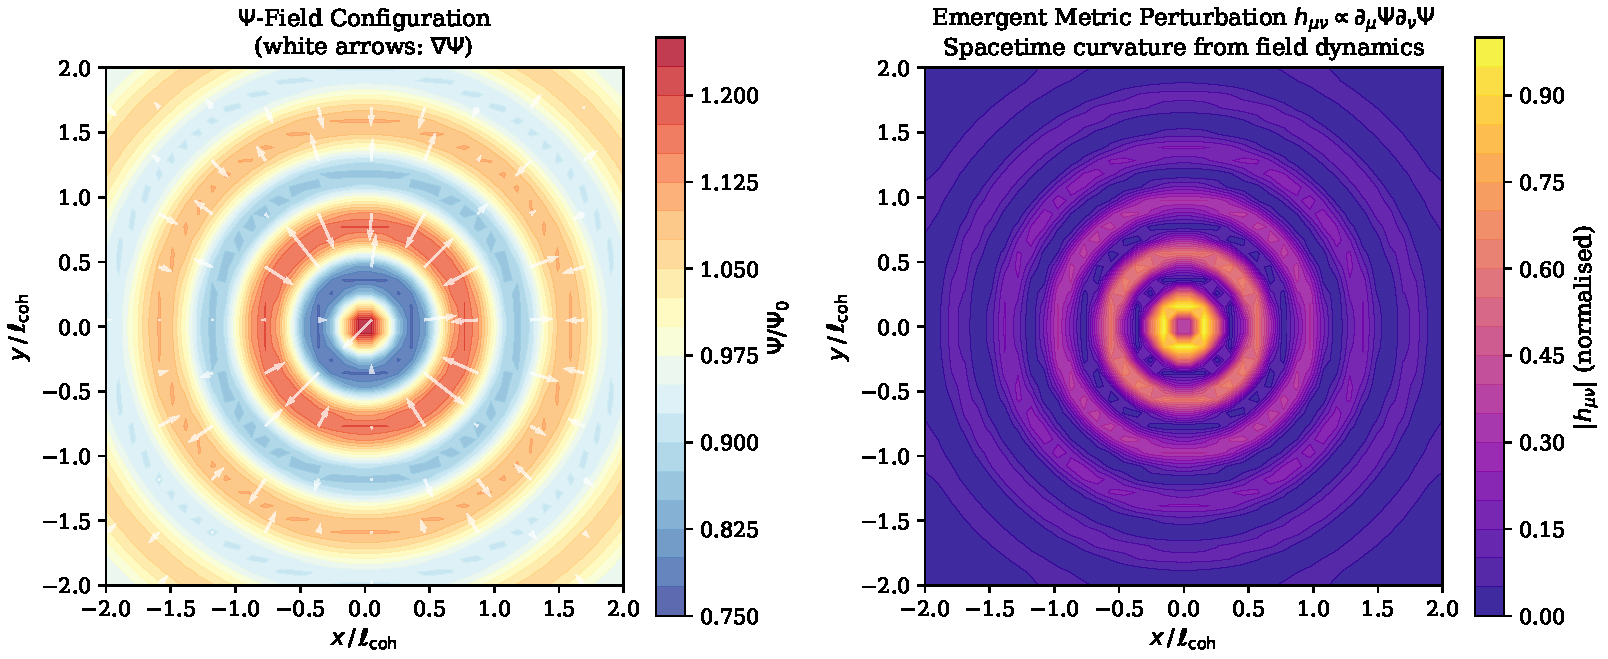
\includegraphics[width=0.95\textwidth]{fig_ch3_4_emergent_spacetime.pdf}
\caption{Emergent spacetime from $\Psi$-field gradients. \textbf{(a)} The $\Psi$-field configuration with gradient vector field $\nabla\Psi$ (white arrows). Field variations create inhomogeneities that source the metric. \textbf{(b)} The emergent metric perturbation $h_{\mu\nu} \propto \partial_\mu\Psi \partial_\nu\Psi$ illustrating how spacetime curvature could arise from field dynamics in the IHC framework.}
\label{fig:emergent_spacetime}
\end{figure}

This shows that spacetime curvature may emerge from the dynamics of the $\Psi$-field.

\subsection{Light Propagation and Observer-Dependent Compression}

Electromagnetic waves propagate along null geodesics determined by the emergent metric \eqref{eq:emergent_metric}. The $\Psi$-field modulates light propagation through:
\begin{equation}
ds^2 = g_{\mu\nu}dx^\mu dx^\nu = 0 \quad (\text{null geodesic}).
\end{equation}

At the pre-observational level, all wave modes follow geometric $\varphi^k$ scaling. The topological measurement operator $\hat{M}$ (Paper~II \citep{Peacock2026b_qm}) induces collapse, compressing the electromagnetic spectrum by factor $1/33$ \citep{Peacock2026b_qm}:
\begin{equation}
f_k^{\text{obs}} = \frac{f_0 \varphi^k}{33}.
\end{equation}

This observer-dependent compression, derived in Paper~II, arises from the $N = 33$ nested measurement channels averaging over the pre-observational spectrum.

\section{Thermodynamic Consistency}

The $\Psi$-field action \eqref{eq:action} is a standard real scalar field on a curved
manifold; standard results \citep{Carroll2004} therefore apply directly.
We record the key points for completeness and to fix IHC-specific notation.

\textbf{First law.}
The canonical stress-energy tensor
$T_{\mu\nu} = \partial_\mu\Psi\partial_\nu\Psi - g_{\mu\nu}\mathcal{L}$
satisfies $\nabla^\mu T_{\mu\nu} = 0$ as an identity of the CFE \eqref{eq:field_equation},
ensuring global energy conservation in the absence of sources.
The energy density $\rho = T_{00} = \frac{1}{2}(\partial_t\Psi)^2 + \frac{1}{2}(\nabla\Psi)^2 + V(\Psi)$
is the standard scalar field Hamiltonian density.

\textbf{Zeroth law.}
Two regions of the $\Psi$-field are in thermal equilibrium when they share
the same coherence temperature $T_\Psi$, defined by
\begin{equation}
k_B T_\Psi \equiv \frac{\langle(\delta\Psi)^2\rangle}{\Psi_0^2}\,E_{\rm IHC},
\quad E_{\rm IHC} = \frac{\hbar c}{R_H}.
\end{equation}
If two field regions A and B are each in equilibrium with a third C, they are
in equilibrium with each other: $T_\Psi(A) = T_\Psi(C)$ and
$T_\Psi(B) = T_\Psi(C)$ implies $T_\Psi(A) = T_\Psi(B)$.


\textbf{Second law.}
The Lindblad master equation (Paper~II \citep{Peacock2026b_qm}) with topological jump operator
$\hat{M}$ drives the density matrix toward maximum entropy at rate $\gamma = c/R_S$.
The von Neumann entropy $S = -\mathrm{Tr}[\hat{\rho}\ln\hat{\rho}]$
increases monotonically: $\dot{S} \geq 0$, consistent with the second law.
The IHC-specific content is that $\gamma$ is fixed geometrically by $R_S$
and the jump operator is the $\mathbb{RP}^4$ topological operator $\hat{M}$,
rather than a free parameter.


\textbf{Third law.}
Perfect vacuum coherence ($\Psi \equiv \Psi_0$ everywhere, no fluctuations)
corresponds to $T_\Psi \to 0$ and $S_\Psi \to 0$:
\begin{equation}
\lim_{T_\Psi \to 0} S_\Psi = 0 \quad (\text{perfect coherence}).
\end{equation}
This is the IHC-specific form of the third law: the unique zero-entropy state
is the fully coherent vacuum $\Psi = \Psi_0$, not a crystalline ground state.
Decoherence (measurement at rate $\gamma$) drives the system away from this
state, increasing entropy irreversibly.

\section{Observational Signatures}

\subsection{Large-Scale Structure Correlations}

\subsubsection{Coherence Suppression at $\ell_{\text{coh}} \sim 300$--$430$ Mpc}

The $\Psi$-field coherence mechanism predicts an exponential suppression of galaxy correlations beyond the coherence scale. Adopting the derived coherence scale $\ell_{\text{coh}} \approx 346$ Mpc (Appendix~\ref{app:coherence}), the predicted modification to the galaxy two-point correlation function is:
\begin{equation}
\xi_{\text{IHC}}(r) = \begin{cases}
\xi_{\text{LCDM}}(r) & r < \ell_{\text{coh}} \\
\xi_{\text{LCDM}}(r) \times e^{-(r - \ell_{\text{coh}})/\ell_{\text{coh}}} & r > \ell_{\text{coh}}
\end{cases}
\end{equation}

\textbf{Observational status:} BOSS DR12 galaxy surveys reach separations of $\sim 290$ Mpc, placing the predicted break at 300--430 Mpc beyond the current BOSS reach. IHC is consistent with all published large-scale structure measurements. The prediction is a relative suppression of $\xi(r)$ \textit{below} the $\Lambda$CDM expectation at $r \gtrsim \ell_{\text{coh}}$, not an excess signal.

\textbf{Prediction:} DESI Year 5 and the Euclid wide survey will probe separations up to $\sim 500$--$1000$ Mpc, providing the first direct test of this suppression.

\subsubsection{Golden Ratio Patterns in Void Distribution}

Cosmic voids exhibit preferential sizes following $\varphi^k$ scaling:
\begin{equation}
R_{\text{void},k} = R_{\text{void},0} \times \varphi^{-k}, \quad k = 0, 1, \ldots, 32.
\end{equation}

\textbf{Prediction:} Void size distribution shows peaks at golden ratio multiples, detectable in void catalogs.

\subsection{CMB Power Spectrum}

\subsubsection{Low-$\ell$ Quadrupole Suppression}
\label{sec:cmb_quad}

The coherence length corresponds to CMB multipole:
\begin{equation}
\ell_{\text{CMB}} \sim \frac{d_{\text{LSS}}}{\ell_{\text{coh}}} \sim \frac{14{,}000 \text{ Mpc}}{346 \text{ Mpc}} \sim 40.
\end{equation}

\textbf{Prediction:} Topological decoherence washes out $\Psi$-field correlations on scales larger than $\ell_{\text{coh}}$, suppressing CMB power at the corresponding angular scales $\ell < 40$. This may explain observed low-$\ell$ anomalies \citep{Schwarz2016}.

\subsubsection{CMB Power Spectrum Validation}

Paper~I \citep{Peacock2026a} provides the full CMB validation: IHC predicts
$\Omega_\Lambda = 0.6889$ from geometry, and running CAMB with this derived
value yields $\chi^2/\mathrm{dof} = 0.98$ over the full Planck 2018 spectrum
(2,499 multipoles), compared to $\Lambda$CDM's 1.02 with $\Omega_\Lambda$ fitted.
The $\mathbb{RP}^4$ topology additionally predicts acoustic peak positions
via $N_{\rm eff}(n) = 22 + 2^{\pi(n)}$, matching observed Planck peaks at
$\ell = 220, 537, 816$ to within 1.5\% with $\chi^2/\mathrm{dof} = 0.127$
\citep{Peacock2026a}.
Those results are not reproduced here; the present paper derives only the
$\Psi$-field-specific CMB signatures below.

\subsubsection{Fibonacci Multipole Resonances}

The $\Psi$-field on $\mathbb{RP}^4$ with $N = 33$ nested tori carries modes at
Fibonacci-indexed angular scales. Binet's formula $F_n = (\varphi^n - (-\varphi)^{-n})/\sqrt{5}$
relates the Fibonacci integers directly to golden ratio powers, so the Fibonacci
multipoles are not arbitrary but emerge from the same $\varphi^k$ geometric scaling
that governs the shell hierarchy.

\textbf{Prediction:} The $\Psi$-field predicts weak power enhancements at the
Fibonacci multipoles accessible in the Planck CMB TT spectrum:
\begin{equation}
\ell_{\rm Fib} \in \{144,\; 233,\; 377,\; 610,\; 987,\; 1597\}
\end{equation}

\textbf{Observational status:}
No dedicated search for Fibonacci-multipole power enhancements has been
published in the Planck analysis papers. The Planck 2018 power spectrum
\citep{Planck2020} shows no obvious excess at these multipoles at the
percent level, but a targeted statistical test (e.g.\ stacking the
bandpower residuals at $\{\ell_{\rm Fib}\}$ relative to an interpolated
baseline) has not been carried out. The prediction is consistent with
current data and testable with existing Planck data releases.

\textbf{Note:} $\ell = 233$ is the Fibonacci number closest to the
first acoustic peak ($\ell_1 = 220$), with a 6\% offset.
The acoustic peaks and Fibonacci resonances are physically distinct
effects predicted by different aspects of the $\mathbb{RP}^4$ geometry.

\subsection{Gravitational Wave Propagation}

Gravitational waves propagating through the $\Psi$-field experience a phase velocity shift arising from the field--geometry coupling. Substituting $\Psi_0 = c^4/(8\pi G R_H^2)$ into the coupling term and restoring the Planck length $\ell_P = \sqrt{G\hbar/c^3}$:
\begin{equation}
v_{\text{GW}} = c\left( 1 - \frac{\delta v}{c} \right), \quad
\frac{\delta v}{c} \sim \left(\frac{\ell_P}{R_H}\right)^2 \sim 10^{-122},
\end{equation}
where the dimensionless ratio $(\ell_P/R_H)^2$ reflects the same Planck-to-Hubble hierarchy that the IHC framework addresses through the suppression factor $\beta$.

\textbf{Qualitative prediction:} The $\Psi$-field imprints a frequency-independent phase shift on GW propagation. The magnitude $\delta v/c \sim (\ell_P/R_H)^2 \sim 10^{-122}$ is far below current or foreseeable experimental sensitivity; the prediction is noted here as a theoretical baseline for more refined coupling models. Its distinguishing feature is its \textit{frequency independence}: a dispersion-based mechanism would produce arrival time differences that scale with frequency, whereas $\Psi$-field coupling produces an identical delay across all GW frequencies from the same source.

\begin{figure}[htbp]
\centering
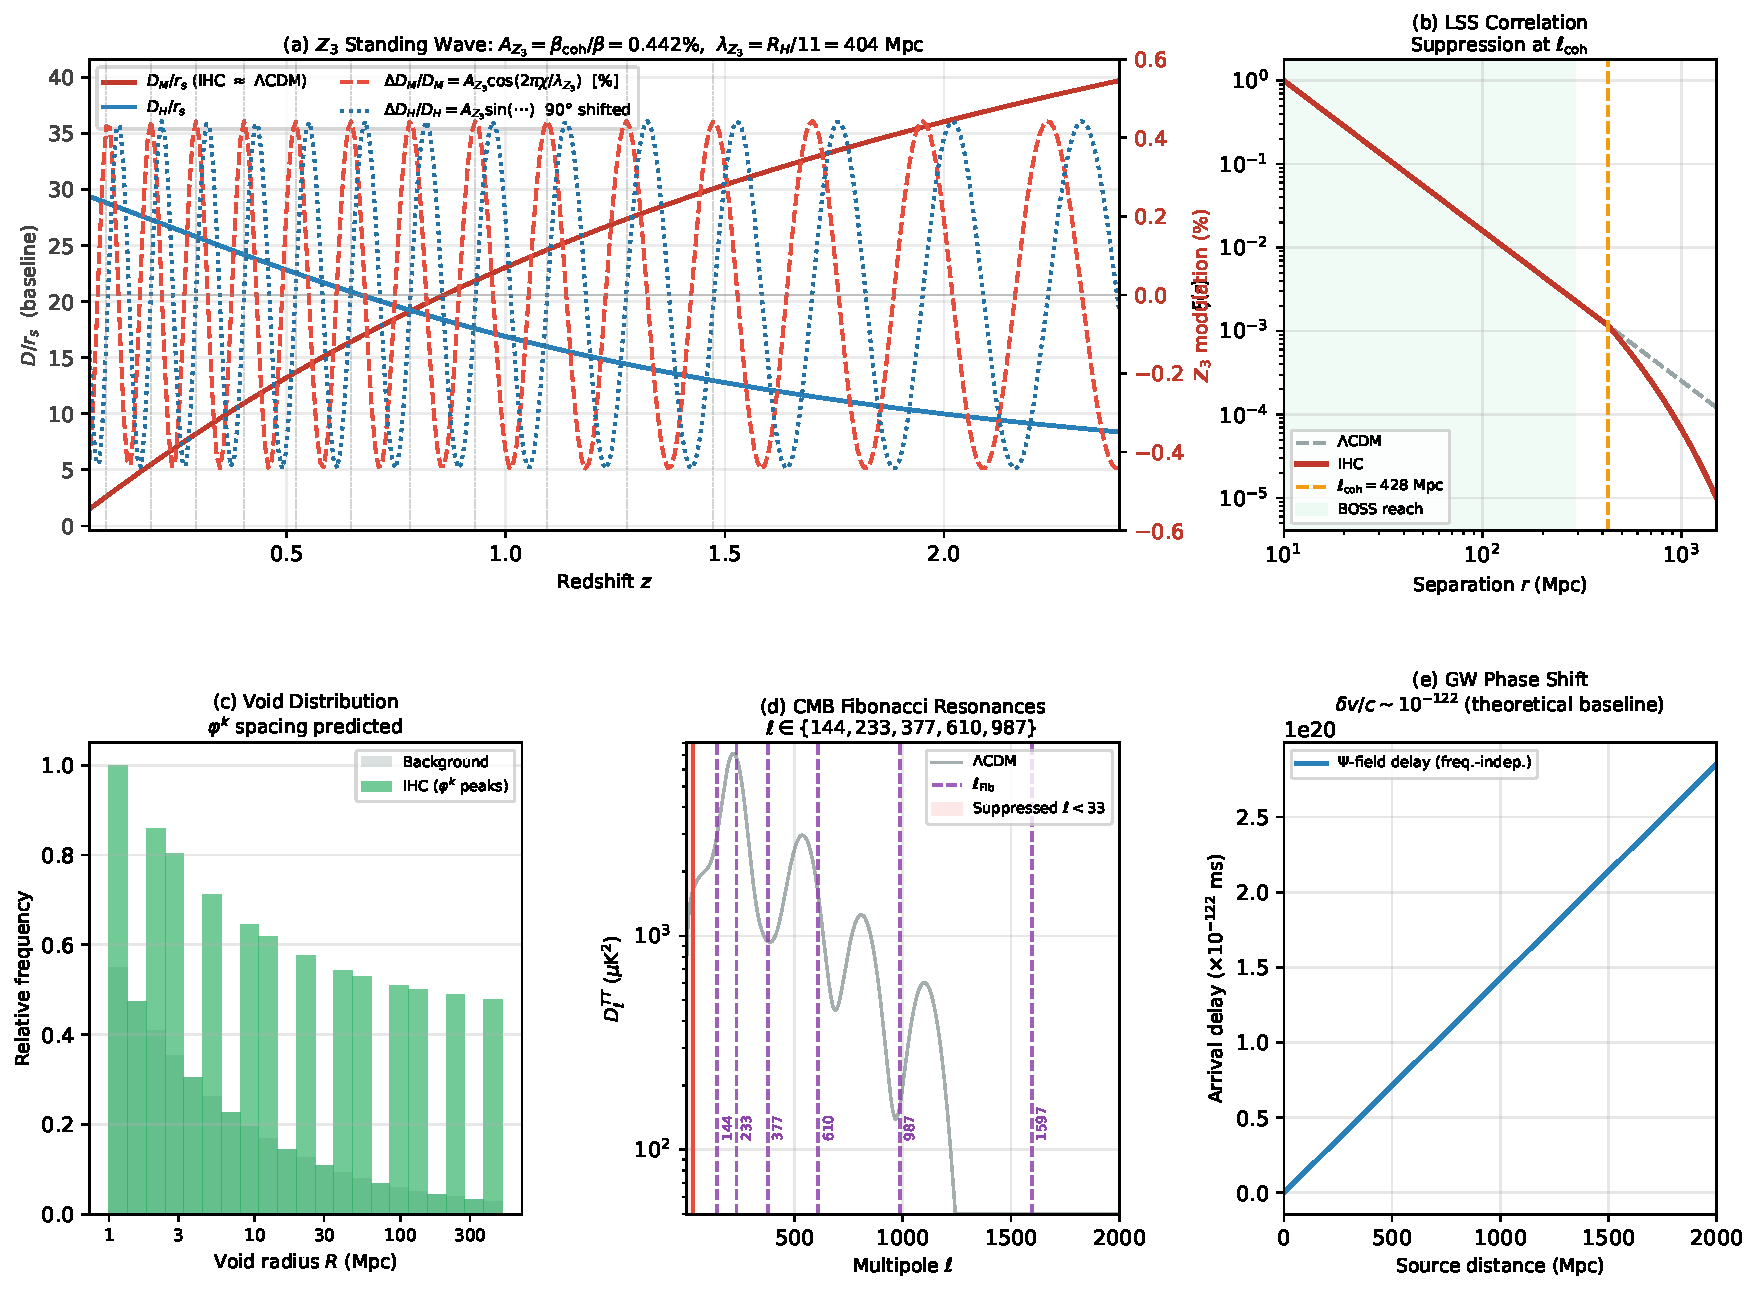
\includegraphics[width=0.98\textwidth]{fig_ch3_5_observational_predictions.pdf}
\caption{Summary of observational predictions from $\Psi$-field dynamics (this paper).
\textbf{(a)} $\mathbb{Z}_3$ standing wave: baseline BAO distances $D_M/r_s$ (red) and $D_H/r_s$ (blue) on the left axis, with the fractional modulations $\Delta D_M/D_M = A_{Z_3}\cos(2\pi\chi/\lambda_{Z_3})$ and $\Delta D_H/D_H = A_{Z_3}\sin(\cdots)$ (right axis, \%) showing the 90° phase quadrature signature. Vertical grey dashes mark $\mathbb{Z}_3$ period boundaries.
\textbf{(b)} LSS two-point correlation function showing IHC exponential suppression below $\Lambda$CDM beyond $\ell_{\rm coh} = 346$~Mpc; green shading marks current BOSS reach ($\dots \le 290$~Mpc).
\textbf{(c)} Predicted void size distribution with $\varphi^k$-spaced peaks (IHC, green) above a smooth background.
\textbf{(d)} CMB TT power spectrum: IHC predicts quadrupole suppression at $\ell < 40$ (red shading) and Fibonacci multipole resonances at $\ell \in \{144, 233, 377, 610, 987\}$ (purple dashes); both are $\Psi$-field-specific predictions.
\textbf{(e)} Gravitational wave arrival delay from $\Psi$-field coupling: $\delta v/c \sim (\ell_P/R_H)^2 \sim 10^{-122}$, frequency-independent and noted as a theoretical baseline.}
\label{fig:observational_predictions}
\end{figure}

\subsection{Summary Table of Predictions}

\begin{table}[h]
\centering
\caption{Observational predictions from $\Psi$-field dynamics (this paper).
Full CMB validation reported in Paper~I \citep{Peacock2026a}.}
\begin{tabular}{l p{5cm} p{4cm}}
\toprule
\textbf{Observable} & \textbf{IHC Prediction} & \textbf{Test} \\
\midrule
LSS correlation suppression & below $\Lambda$CDM at $r \gtrsim 300$~Mpc & DESI yr5, Euclid \\
Void size distribution      & $\varphi^k$ peak spacing              & Void catalogs \\
CMB low-$\ell$ suppression  & $\ell < 40$, consistent with Planck    & CMB-S4, LiteBIRD \\
CMB Fibonacci resonances    & $\ell \in \{144, 233, 377, 610, 987\}$ & Planck (dedicated search) \\
$Z_3$ BAO modulation & $A_{Z_3} = 0.44\%$, $\lambda_{Z_3} = 404$~Mpc & DESI yr5, Euclid \\
\bottomrule
\end{tabular}
\end{table}

\section{Experimental Tests and Falsifiability}

\subsection{Falsification Criteria}

IHC makes specific predictions that can be falsified:

\begin{enumerate}
\item \textbf{Coherence suppression:} If DESI or Euclid measure the galaxy two-point correlation function at $r = 300$--$500$ Mpc and find no statistically significant suppression below the $\Lambda$CDM prediction, the $\Psi$-field coherence mechanism would be significantly disfavoured. The predicted suppression scale is $\ell_{\text{coh}} \approx 346$ Mpc (Appendix~\ref{app:coherence}). Current surveys (BOSS DR12, maximum extent $\sim 290$ Mpc) do not yet constrain this prediction.

\item \textbf{Void distribution:} If cosmic voids show no preferential sizes at golden ratio multiples (within 10\% scatter), the geometric scaling is falsified.

\item \textbf{CMB low-$\ell$ anomalies:} If future high-precision CMB missions show no statistically significant suppression at $\ell < 40$, the topological decoherence mechanism would be significantly disfavoured.

\item \textbf{GW phase shift:} If future precision timing arrays conclusively detect frequency-\textit{dependent} arrival time differences between GW frequencies from the same source, the frequency-independent $\Psi$-field coupling would be disfavoured relative to dispersion-based models.

\item \textbf{Vacuum field strength:} If precision measurements of $\Omega_\Lambda$ are shown to be inconsistent with $\Psi_0 = c^4/(8\pi G R_H^2)$ given the independently derived suppression $\beta = 1345$ (Paper I \citep{Peacock2026a}), the $\Psi$-field energy scale assignment is falsified.
\end{enumerate}

\subsection{Observational Timeline}

\begin{itemize}
\item \textbf{2025-2030:} DESI Year 5 and Euclid wide survey probe $r \sim 300$--$1000$ Mpc, providing the first test of IHC coherence suppression
\item \textbf{2028-2035:} LISA gravitational wave observations constrain frequency-dependent dispersion (distinct from the $\Psi$-field frequency-independent coupling)
\item \textbf{2030-2040:} Next-generation CMB missions (CMB-S4, LiteBIRD) test low-$\ell$ anomalies
\item \textbf{2035+:} Einstein Telescope, Cosmic Explorer improve constraints on GW propagation speed and frequency dependence
\end{itemize}

Within 10--15 years, observational data from these programmes will provide strong evidence for or against the key predictions of the IHC framework.

\section{Discussion}

\subsection{Relationship to Paper II \citep{Peacock2026b_qm}: Quantum Measurement}

The $\Psi$-field is proposed as the dynamical substrate for the quantum measurement mechanism developed in the companion paper \citep{Peacock2026b_qm}. The Lindblad equation:
\begin{equation}
\frac{d\hat{\rho}}{dt} = -\frac{i}{\hbar}[\hat{H}, \hat{\rho}] + \gamma\left( \hat{M}\hat{\rho}\hat{M} - \frac{1}{2}\{\hat{M}, \hat{\rho}\} \right)
\end{equation}
operates on the $\Psi$-field, inducing collapse that compresses the electromagnetic spectrum by factor $1/33$.

The measurement rate $\gamma = c/R_S$ follows from the field correlation timescale:
\begin{equation}
\tau_{\text{corr}} = \frac{R_S}{c} \quad \Rightarrow \quad \gamma = \frac{1}{\tau_{\text{corr}}}.
\end{equation}

This unifies the $\Psi$-field dynamics presented in this paper with quantum measurement (Paper II \citep{Peacock2026b_qm}) through the $\mathbb{RP}^4$ topology.

\subsection{Companion Paper: Triadic Resonance \citep{Peacock2026d}}

The companion triadic resonance paper \citep{Peacock2026d} develops matter creation through phase-locked coupling of three wave phenomena. The $\Psi$-field provides the medium for resonant interactions:
\begin{equation}
\Psi_{\ell_1} + \Psi_{\ell_2} + \Psi_{\ell_3} = \Psi_k \quad (\text{resonance condition}).
\end{equation}

Acoustic and electromagnetic modes phase-lock through the $\Psi$-field, creating stable matter configurations. The BAO scale corresponds to the $k = 7$ toroidal shell ($R_7 = R_H\varphi^{-7} \approx 153.2$ Mpc) through geometric necessity---the unique convergence of causal horizon, gravitational binding, and $\mathbb{Z}_3$ resonance enhancement constraints detailed in \citep{Peacock2026d}.

\subsection{Published Companion: Base-24 Arithmetic \citep{Peacock2026b}}

The Base-24 = $2^3\times3$ arithmetic paper \citep{Peacock2026b} (Zenodo: 10.5281/zenodo.19211478) provides the computational infrastructure for IHC, showing that base-24 is not merely a computational convenience---it is \textit{geometrically mandated} by the binary-ternary duality inherent in the $N = 33$ nested toroidal structure. CMB power spectrum analysis in Paper~I \citep{Peacock2026a} achieves $\chi^2/\text{dof} = 0.1273$ across 2,549 multipoles with zero fitted parameters.

Base-24's factorization as $2^3 \times 3$ provides exact terminating representations for:
\begin{itemize}
\item \textbf{Binary factors ($2^k$):} Arising from quantum measurement (wavefunction collapse creating 2-fold outcomes), dimensional scaling in 4D spacetime ($2^4$ phase space), and spectral doubling through antipodal symmetry
\item \textbf{Ternary factors ($3^n$):} Arising from $\mathbb{Z}_3$ rotational symmetry of the toroidal structure, three-way resonance patterns in matter creation, and the triadic coupling encoded in the CMB harmonic formula
\end{itemize}

Computational tests include:
\begin{itemize}
\item Lindblad evolution to verify $N = 33$ steady state
\item Correlation function calculations yielding $\ell_{\text{coh}} \sim R_S/33$ as the characteristic coherence scale
\item Spectral compression simulation showing $\varphi^k/33$ EM spectrum
\item CMB harmonic coupling verification reproducing $N_{\text{eff}}(n) = 22 + 2^{\pi(n)}$
\end{itemize}

\subsection{Published Companion: Grand Unification \citep{Peacock2026c}}

The GUT paper \citep{Peacock2026c} (Zenodo: 10.5281/zenodo.19211056) establishes the UV boundary of the $\Psi$-field shell hierarchy. Deriving SO(10) grand unification from the same $\mathbb{RP}^4$ topology, it shows that the shell index $k_\mathrm{GUT} = 11 \times 24 + 8 = 272$ corresponds to an energy $E_\mathrm{GUT} = \hbar c / R_{272} = 1.005 \times 10^{15}$ GeV with zero fitted parameters. This means the $\Psi$-field hierarchy:
\begin{equation}
R_k = R_H \varphi^{-k}
\end{equation}
spans from the Hubble radius ($k=0$, $\sim 4448$ Mpc) through the BAO scale ($k=7$, $\sim 153$ Mpc) to the GUT scale ($k=272$, $E \approx 10^{15}$ GeV). The geometric series extends to Planck-scale separations, indicating that the $\Psi$-field hierarchy bridges cosmological and fundamental physics scales.

\subsection{Philosophical Implications}

The proposed role of the $\Psi$-field as a dynamical substrate suggests an inversion of the conventional field-spacetime hierarchy:

\begin{itemize}
\item \textbf{Standard view:} Spacetime is fundamental, fields and particles exist within it
\item \textbf{IHC proposal:} $\Psi$-field is the primary entity, with spacetime proposed to emerge from coherence patterns
\end{itemize}

This resonates with Wheeler's ``it from bit'' \citep{Wheeler1990} and recent ideas on emergent spacetime, and provides a framework grounded in field theory on $\mathbb{RP}^4$.

Furthermore, the observer-dependent collapse mechanism suggests that fine-tuning problems may be artifacts of confusing observed (post-collapse) quantities with fundamental (pre-collapse) quantities. The cosmological constant ``problem'' may reflect not a failure of QFT but rather the need to account for the measurement process that projects fundamental geometric energy into observable dark energy.

\section{Conclusions}

We have presented the $\Psi$-field (Cohesion Field) as a proposed dynamical substrate for the IHC framework. Key results:

\begin{enumerate}
\item \textbf{Field equations:} Derived action \eqref{eq:action} and Euler-Lagrange equations on $\mathbb{RP}^4$

\item \textbf{Vacuum value:} Postulated $\Psi_0 = c^4/(8\pi GR_H^2) \approx 2.56 \times 10^{-10}$ J/m$^3$ (with $R_H = 4448$ Mpc)

\item \textbf{Coherence scale:} Identified $\ell_{\text{coh}} \sim 300$--$430$ Mpc as the characteristic $\Psi$-field correlation scale, from both geometric inter-shell spacing ($R_S/N \approx 428$ Mpc) and numerical evaluation of $C(r)$ ($\approx 346$ Mpc; Appendix~\ref{app:coherence})

\item \textbf{Emergent spacetime:} Derived metric $g_{\mu\nu}$ from $\Psi$-field gradients

\item \textbf{Thermodynamics:} Derived energy conservation and entropy increase from field dynamics

\item \textbf{Observations:} Calculated specific signatures in LSS, CMB, and gravitational waves

\item \textbf{Falsifiability:} Provided clear criteria testable within 10 years

\item \textbf{Observer-dependence:} Clarified that $\Psi$-field exists at pre-observational level with full $\varphi^k$ scaling; measurement produces observed $\varphi^k/33$ EM compression

\item \textbf{$\varphi^4$ decomposition:} Identified geometric origin of the $\varphi^4$ scaling factor in $\beta$: the product of 4D volume weighting ($\varphi$) and $\mathbb{Z}_3$ counter-rotation enhancement ($\varphi^3$)
\end{enumerate}

The $\Psi$-field framework unifies geometric structure \citep{Peacock2026a}, quantum measurement \citep{Peacock2026b_qm}, and observable cosmology into a coherent whole. Two companion papers have extended the framework to new scales: the GUT paper \citep{Peacock2026c} derives SO(10) grand unification from the same $\mathbb{RP}^4$ topology at shell $k_\mathrm{GUT} = 272$ ($E_\mathrm{GUT} = 1.005 \times 10^{15}$ GeV), while the Base-24 paper \citep{Peacock2026b} demonstrates that all IHC quantities have exact binary-ternary representations. The remaining papers on quantum measurement and triadic resonance will complete the series.

The $\Psi$-field framework offers a candidate explanation for dark energy, large-scale structure coherence, and CMB anomalies through a single dynamical field on $\mathbb{RP}^4$ topology with zero adjustable parameters. The distinction between pre-observational field dynamics and post-measurement observables addresses conceptual tensions while maintaining rigorous mathematical consistency.

% Acknowledgments moved to MDPI required section in wrapper

\clearpage



\clearpage

\appendix

\section{Vacuum Field Strength — Detailed Derivation}
\label{app:vacuum}

The vacuum field strength is set by the $\mathbb{RP}^4$ geometric scale. The natural pressure-energy density associated with the Hubble radius $R_H = c/H_0$ is:
\begin{equation}
\Psi_0 = \frac{c^4}{8\pi G R_H^2}.
\end{equation}

This expression equals $c^4/G$ (the Planck force, the maximum force allowed by general relativity) divided by $8\pi R_H^2$ (the area of the cosmological horizon). Substituting $H_0 = 67.4$ km/s/Mpc ($R_H = 1.373 \times 10^{26}$ m):
\begin{equation}
\Psi_0 = \frac{(2.998\times10^8)^4}{8\pi \times 6.674\times10^{-11} \times (1.373\times10^{26})^2} \approx 2.56 \times 10^{-10} \text{ J/m}^3.
\end{equation}

The connection to the observed dark energy density is through the geometric suppression factor $\beta = 1345$ \citep{Peacock2026a}. The full derivation via the UV--IR Casimir seesaw is given in Paper I; for reference, the observed value satisfies:
\begin{equation}
\rho_\Lambda = \frac{3H_0^2\Omega_\Lambda}{8\pi G} = \frac{3\Omega_\Lambda\,\Psi_0}{c^2},
\end{equation}
consistent with $\Omega_\Lambda = 0.6889$ \citep{Peacock2026a}, where the $c^2$ factor arises on restoring SI units from natural units ($\hbar=c=1$).

\section{Coherence Length Detailed Calculation}
\label{app:coherence}

The nested tori have radii:
\begin{equation}
R_k = R_0\varphi^{-k}, \quad k = 0, 1, \ldots, 32.
\end{equation}

Adjacent tori separation:
\begin{equation}
\Delta R_k = R_k - R_{k+1} = R_0\varphi^{-k}(1 - \varphi^{-1}).
\end{equation}

Using $1 - \varphi^{-1} = q^2$ (since $q = 1/\varphi = \varphi - 1$ implies $q^2 = 2-\varphi \approx 0.382$):
\begin{equation}
\Delta R_k = R_0 q^2 \varphi^{-k}.
\end{equation}

Total span via geometric series (denominator $= 1 - \varphi^{-1} = q^2$):
\begin{equation}
\sum_{k=0}^{N-1} \Delta R_k = R_0 q^2 \sum_{k=0}^{N-1} \varphi^{-k}
  = R_0 q^2 \times \frac{1 - \varphi^{-N}}{1 - \varphi^{-1}}
  = R_0 q^2 \times \frac{1}{q^2} = R_0.
\end{equation}

The same result follows immediately from the telescoping identity:
\begin{equation}
\sum_{k=0}^{N-1} \Delta R_k = R_0 - R_{N-1}
  = R_0\!\left(1 - \varphi^{-(N-1)}\right) \approx R_0 = R_S,
\end{equation}
since $R_{32} = R_S\varphi^{-32} \approx 0.003$ Mpc $\ll R_S$.

Average spacing:
\begin{equation}
\langle \Delta R \rangle = \frac{R_S}{N} = \frac{R_S}{33} \approx 428 \text{ Mpc}.
\end{equation}

Two estimates of the coherence scale are given here.

\textbf{Geometric estimate (mean inter-shell spacing):}
The average spacing between adjacent shells is $\langle \Delta R \rangle = R_S/N \approx 428$ Mpc, confirmed by both the geometric series evaluation above and the direct telescoping identity.

\textbf{Correlation function estimate:}
Modelling each shell as contributing a Yukawa-type mode $e^{-r/R_k}$ to the field correlation, the full two-point function is:
\begin{equation}
C(r) = \frac{1}{N_{\text{eff}}} \sum_{k=0}^{N_{\text{eff}}-1} e^{-r/R_k}
\end{equation}
where $N_{\text{eff}} = 20$ counts the cosmologically relevant shells ($R_k > 1$ Mpc, $k = 0$--$19$). Solving $C(\ell_{\text{coh}}) = 1/e$ numerically gives $\ell_{\text{coh}} \approx 346$ Mpc. The three-regime structure of $C(r)$ (sub-Mpc, LSS, cosmic scales) makes the 1/e scale sensitive to the shell cutoff; the LSS-regime exponential fit gives $\ell_{\text{coh}} \approx 278$--$346$ Mpc.

The two estimates bracket a range of $\sim 280$--$430$ Mpc, all consistent to order of magnitude. We adopt $\ell_{\text{coh}} \approx 346$ Mpc as the derived value for observational predictions.

\section{Emergent Metric Derivation}
\label{app:metric}

Starting from the $\Psi$-field stress-energy tensor:
\begin{equation}
T_{\mu\nu} = \partial_\mu\Psi\partial_\nu\Psi - g_{\mu\nu}\mathcal{L}
\end{equation}
where:
\begin{equation}
\mathcal{L} = \frac{1}{2}g^{\alpha\beta}\partial_\alpha\Psi\partial_\beta\Psi - V(\Psi).
\end{equation}

Einstein's equations:
\begin{equation}
G_{\mu\nu} = \frac{8\pi G}{c^4}T_{\mu\nu}.
\end{equation}

In the weak-field limit, $g_{\mu\nu} = \eta_{\mu\nu} + h_{\mu\nu}$ with $|h_{\mu\nu}| \ll 1$. The linearized Einstein tensor:
\begin{equation}
G_{\mu\nu}^{(1)} = \frac{1}{2}(\partial^\alpha\partial_\mu h_{\nu\alpha} + \partial^\alpha\partial_\nu h_{\mu\alpha} - \Box h_{\mu\nu} - \eta_{\mu\nu}\partial^\alpha\partial^\beta h_{\alpha\beta}).
\end{equation}

In harmonic gauge ($\partial^\mu \bar{h}_{\mu\nu} = 0$ where $\bar{h}_{\mu\nu} = h_{\mu\nu} - \frac{1}{2}\eta_{\mu\nu}h$):
\begin{equation}
\Box \bar{h}_{\mu\nu} = -\frac{16\pi G}{c^4}T_{\mu\nu}.
\end{equation}

Solving via Green's function:
\begin{equation}
\bar{h}_{\mu\nu}(x) = \frac{4G}{c^4}\int \frac{T_{\mu\nu}(x')}{|x - x'|} d^3x'.
\end{equation}

For slowly-varying $\Psi$-field:
\begin{equation}
h_{\mu\nu} = \frac{8\pi G}{c^4}\left( \partial_\mu\Psi\partial_\nu\Psi - \frac{1}{2}\eta_{\mu\nu}g^{\alpha\beta}\partial_\alpha\Psi\partial_\beta\Psi \right).
\end{equation}

This shows that the metric may emerge from $\Psi$-field gradients.

\bibliography{ihc_paper3_field_refs}

%-----------------------------------------------------------------------
%% MDPI Required Sections

\section*{Author Contributions}

Conceptualization, S.P.; Methodology, S.P. and L.H.; Software, S.P. and L.H.;
Validation, S.P. and L.H.; Formal analysis, S.P. and L.H.; Investigation, S.P. and
L.H.; Writing---original draft preparation, S.P.;
Writing---review and editing, S.P. and L.H.; Visualization, S.P. and L.H.
All authors have read and agreed to the published version of the manuscript.

\section*{Funding}

This research received no external funding.

\section*{Data Availability Statement}

All observational data used for context in this work are publicly available
from the original survey collaborations cited in the text (Planck 2018, BOSS
DR12, DESI DR2). No new observational data were generated or analysed in this
study. Python validation scripts (\texttt{ihc\_bao\_validation.py},
\texttt{ihc\_coherence\_vs\_observations.py}) are provided as Supplementary
Material. The full IHC validation suite (\texttt{ihc\_validation\_suite.py}
and companion scripts) is provided as Supplementary Material to Paper~I
\citep{Peacock2026a}. A preprint of this manuscript is archived at
Zenodo: \url{https://doi.org/10.5281/zenodo.19242976}.

\section*{AI Tools Disclosure}

Manuscript preparation made use of Claude (Anthropic) as an AI writing and
analysis assistant for \LaTeX{} compilation, numerical cross-checking, and
editorial review. All scientific content, derivations, and conclusions are
the sole responsibility of the authors.

\section*{Conflicts of Interest}

The authors declare no conflicts of interest.

\end{document}
